\chapter{CC-Inclusive Cross Section Selection Filter} \label{ch:meas}
The CC-Inclusive cross-section selection I and selection I modified filters used in this analysis will be described in the following sections below. These filters are an expansion of the Neutrino ID filter. The work done in this thesis was to further improve these selections by increasing both efficiency and purity as well as increasing acceptance without further affecting the kinematic distributions of the selected neutrino events.
 
MicroBooNE requires fully automated event reconstruction and selection algorithms for use in the many physics measurements being worked on to date due to the large data rate MicroBooNE receives. Being able to automatically pluck out the neutrino interaction among a sea of cosmics proved to be challenging but was accomplished. MicroBooNE has developed two complementary and preliminary selection algorithms to select charged-current $\nu_{\mu}-Ar$ interactions. Both are fully automated and cut based. The results of this thesis will focus on selection I and selection I modified and will focus on further improving these algorithms using Convolutional Neural Network (CNN) implementations. These selections identify the muon from a neutrino interaction without biasing towards track multiplicity. To combat cosmic and neutral current background, the analysis is strongly biased towards forward-going long tracks which are contained. This limits phase space and reduces acceptance. 

\section{Data and MC Processing Chain}
The data used for this analysis were based on hardware and software triggers. Events used came from the \textit{BNB\_INCLUSIVE} and \textit{EXT\_BNB\_INCLUSIVE} streams and were used for signal and background. The \textit{BNB\_INCLUSIVE} stream is chosen by requiring that the hardware trigger bit is fired and that the event passed an optical software trigger within a BNB spill timing window. The \textit{EXT\_BNB\_INCLUSIVE} stream requires the EXT hardware trigger to fire as well as pass the same optical software trigger within a BNB spill size timing window similar to the \textit{BNB\_INCLUSIVE}. 

The two MC samples used in this analysis and for determining selection efficiencies and purities were GENIE BNB neutrino interactions with CORSIKA cosmic ray overlay within the readout window and inTime CORSIKA cosmic rays. The MC samples generated used \textit{\textbf{uboonecode v04\_36\_00}} and are based on the following packages:
\begin{itemize}
\item{larsoft v04\_36\_00}
\item{GEANT v04\_09\_06\_p04d}
\item{GENIE v02\_08\_06d}
\item{GENIE xsec v02\_08\_06a}
\item{pandora v02\_03\_0a}
\item{CORSIKA v07\_4003}
\end{itemize}

Both data and MC samples were processed using the same reconstruction release, \textit{\textbf{uboonecode v05\_08\_00}} and the fcl files used for reconstruction are listed below:
\begin{itemize}
\item{MC fcl files}
\begin{itemize}
\item{reco\_uboone\_mcc7\_driver\_stage1.fcl}
\item{reco\_uboone\_mcc7\_driver\_stage2.fcl}
\end{itemize}
\item{Data fcl files}
\item{reco\_uboone\_data\_Feb2016\_driver\_stage1.fcl}
\item{reco\_uboone\_data\_Feb2016\_driver\_stage2.fcl}
\end{itemize}

On top of the hardware and software triggers, the data also had to pass more criteria to be identified as part of the good run list. The criteria is detailed below.
\begin{itemize}
\item{\textbf{Detector conditions:} the detector has to be in a good operating condition. The detector conditions are read from the slow monitoring database and are required to be within the alarm thresholds. The variables of interest for events passing the good run list criteria include DAQ, PMT, HV, Drift HV, wire bias, electron lifetime and detector power. These conditions need to be met on a run-by-run basis in order to pass the selection.}
\item{\textbf{Data quality:} normal and stable behavior for basic reconstruction quantities. These reconstruction variables include average number of tracks, hits, and flashes in each event, the average length of tracks, the average amplitude and area of hits, the average PE and the average spread of each one of these quantities.}
\item{\textbf{Beam Conditions:} the BNB must be on and stable and the POT per spill needs to above the intensity threshold. Beam quality conditions include checking the fraction of proton beam interacting within the target, the horn current, and the intensity of protons per spill. The final sample is $5 * 10^{19}$ and a per-spill intensity of $4 * 10^{12}$}
\item{\textbf{Run processed:} the full run must be processed completely without missing subruns or crashes in the data processing.}
\end{itemize}

\section{Normalization of data and MC}\label{section:normalize}
The off-beam sample is used to measure beam unrelated backgrounds. For normalization, one needs the total number of BNB spills \textit{$(N_{BNB}$} and the total number of external triggers. The BNB spills used need to pass the beam quality cuts. The normalization factor is then \textit{$N_{BNB}/N_{EXT}$} which is 1.23. 

To normalize generated BNB MC events to POT, we used the following:
\begin{itemize}
\item{ $5 * 10^{19} POT = 41524.3$ generated events}
\end{itemize}
where this scaling factor only applies to mcc7 generated events. The inTime cosmic sample is normalized with respect to the open cosmic sample so an understanding of both is necessary. The POT per beam spill for mcc7 BNB samples is $5 * 10^{12}$. To calculate how many spills are necessary to produce a specific POT one would multiply the total POT by the average 1/POT per spill. For a total POT of $5 * 10^{19}$ the amount of spills necessary is $\frac{5 * 10^{19}}{5 * 10^{12}} = 1 * 10^7$. This is only one in \sim 241 events therefore each cosmic event needs to be scaled up by a factor of 240.8 when comparing to BNB MC. For inTime cosmics however, two filters are applied to reduce computing and processing time and only leave cosmics that will interact within the detector. The passing rate after these two filters is 0.02125, therefore the total inTime cosmic scaling factor to compare inTime cosmics to BNB is $0.02125 * 240.8 = 5.12$.

%The efficiency and purity are used as performance values of selection I. Efficiency is described as the number of selected true $\nu_{\mu}$ CC events divided by the number of expected true $\nu_{\mu}$ CC events. The purity is described as the number of selected true $\nu_{\mu}$ CC events divided by the sum of itself and all the backgrounds. The efficiency of selection I is 12\% and the purity is 39.7\%. The poster related to this proceedings will focus on the last cut which requires the longest track to be longer than 75 cm. This cut has a passing rate of 30\% w.r.t the previous cut and is implemented in part to separate charged-current events from neutral-current events that mimic our signal. Implementing a CNN for $\mu-\pi$ separation picks out differences in these two particles that are track range independent therefore eliminating the need for the 75 cm track length cut and increase efficiency and passing rate at low muon momentum. Figure \ref{fig:track} shows the track distribution of selection I and the lack of data below  the 75 cm track length cut. Figure \ref{fig:eff} shows the efficiency of selection I as a function of muon momentum.     
\begin{figure}[htp!]
\centering
	\begin{subfigure}[b]{.4\textwidth}
	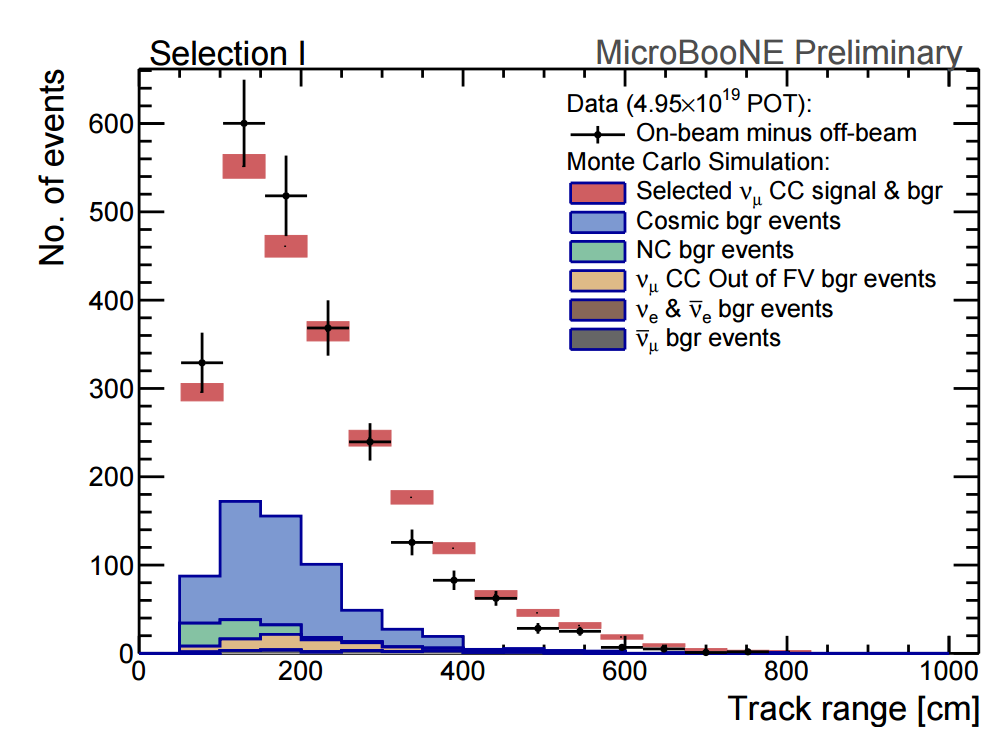
\includegraphics[width=\textwidth]{figs/track_distribution.png}
	\caption{Track range distribution of selection I}
	\label{fig:track}
	\end{subfigure}
	\quad	
	\begin{subfigure}[b]{.4\textwidth}
	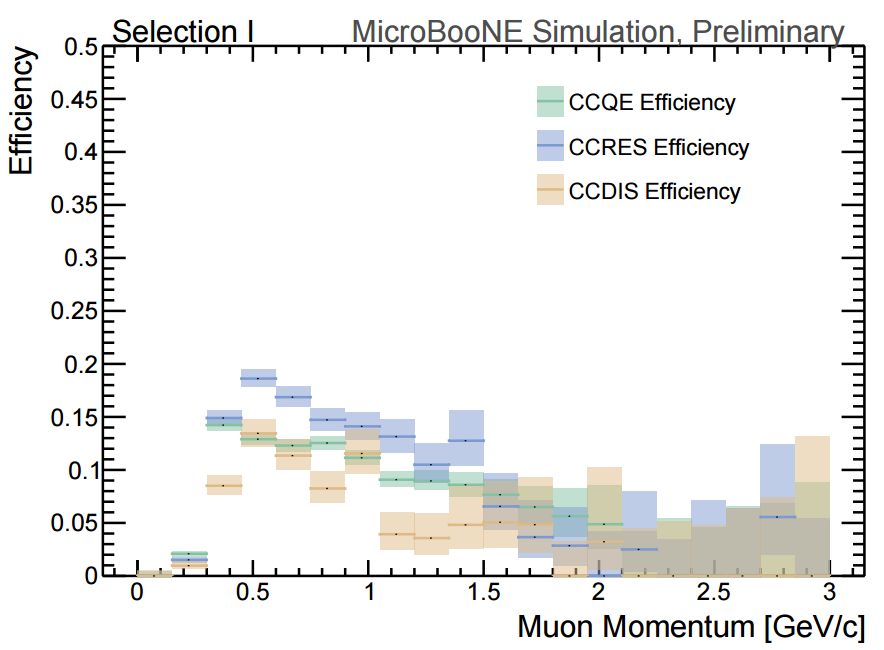
\includegraphics[width=\textwidth]{figs/efficiencyvsmom.png}
	\caption{Selection efficiency as a function of the true muon momentum}
	\label{fig:eff}
	\end{subfigure}
	\quad
\label{fig:distributions}
\caption{\ref{fig:track} Track range distribution for selection I. The track range is defined as the 3D distance between the start and end of the muon candidate track. No data is shown below 75 cm due to the track length cut described previously. \ref{fig:eff} Efficiency of the selected events by process quasi-elastic (QE), resonant (RES), and deep-inelastic (DIS). Statistical uncertainty is shown in the bands and the distributions are a function of true muon momentum. The rise of the efficiency between 0 GeV and 0.5 GeV is due to the minimum track length cut and the decreasing efficiency for higher momentum tracks is caused by the containment requirement.} 
\end{figure}
\section{Optical Software Trigger and Reconstruction}
\subsection{Software Trigger}
Most of the BNB spills from the accelerator do not have a neutrino interaction in MicroBooNE. To save computation resources and reduce data-rates, we require a burst of light in the light collection system in coincidence with the 1.6 $\micro s $ beam spill. Requiring light activity in coincidence with the beam spill eliminates the vast majority of triggers with no neutrino interaction in the detector, however, it doesn't guarantee the activity in the detector is a neutrino interaction since a cosmic ray can interact in coincidence with the beam spill as well.

To implement this, a software trigger was used on the PMT waveforms to decide whether or not to keep that event. The software trigger is implemented after the event builder combines data from the PMTs and triggers into a single event. The software trigger uses the digitized output of the 32 PMT channels in the light collection system. Only the waveform region in coincidence with the beam spill is used to search for possible triggers. For each PMT, a waveform is found by taking the difference of ADC values is calculated between \textit{t} and \textit{t + s}. This waveform is then scanned for ADC values above a threshold \textit{$X_0$}. Once an ADC is above this threshold, a discriminator window is opened for a fixed number of time ticks \textit{($W_0$)}. If the ADC count within this window \textit{$W_0$} is greater than a second larger threshold \textit{$X_3$}, a final window of width \textit{$W_3$} is opened. The max ADC value within this final window is set as the peak amplitude for the PMT and then summed across all 32 PMTs and set to the variable PHMAX. The software trigger places a final cut on the PHMAX variable to decide whether or not to keep the event. The thresholds were found by the Trigger task force using Monte Carlo Studies 
and are as follows: 
\begin{itemize}
\item{$X_0$ = 5 ADC} 
\item{$X_3$ = 10 ADC} 
\item{$W_0$ = 6 Ticks} 
\item{$W_3$ = 6 Ticks} 
\item{PHMAX cut = 130 ADC}
\end{itemize}

\subsection{Flash Reconstruction}
MicroBooNE collects light from each of the 32 PMTs either in a continuous readout window of 23.4 $\micro S$ activated by a beam gate signal on the trigger board, or in discriminated pulses of \sim 1 $\micro s$ duration activated if the ADC count for any PMT goes above 80 ADC count. These two formats are saved as output waveforms and put onto an event. Additionally, each PMT can provide two output streams, high-gain (\sim 20 ADC/PE) and low-gain (\sim 2 ADC/PE) channels. The first step in the reconstruction is to merge both these channels into a ``saturation corrected waveform'' which uses information from the low-gain waveform to correct for saturating high-gain pulses.
 
The saturation corrected waveform in the continuous readout window is used to reconstruct optical hits. Each PMT's waveform is scanned for hits then a threshold based hit reconstruction algorithm is applied which requires pulses of a minimum area in order to be reconstructed. Each reconstructed hit is associated to a PMT, a time in $\micro s$, and a PE count. 

Once hits are reconstructed for all 32 PMTs, all PMT information is then combined into optical flashes which represent optical information seen by the PMTs from interactions in the detector. Each flash has information on total light seen per interaction,  the distribution of the light across all 32 PMTs, the flash time with respect to the trigger time of the flash, and lastly, the spacial information of the flash in Y-Z plane of the detector. These flashes are reconstructed by requiring that there is a \sim 1 $\micro s$ coincidence between the reconstructed hits in all 32 PMTs. The total PE is summed up among all coincident hits across the PMTs and if the total PE is greater than 2 PE, a flash is reconstructed. There are also safe guards in place to take care of late scintillation light.  

\begin{figure}[htp!]
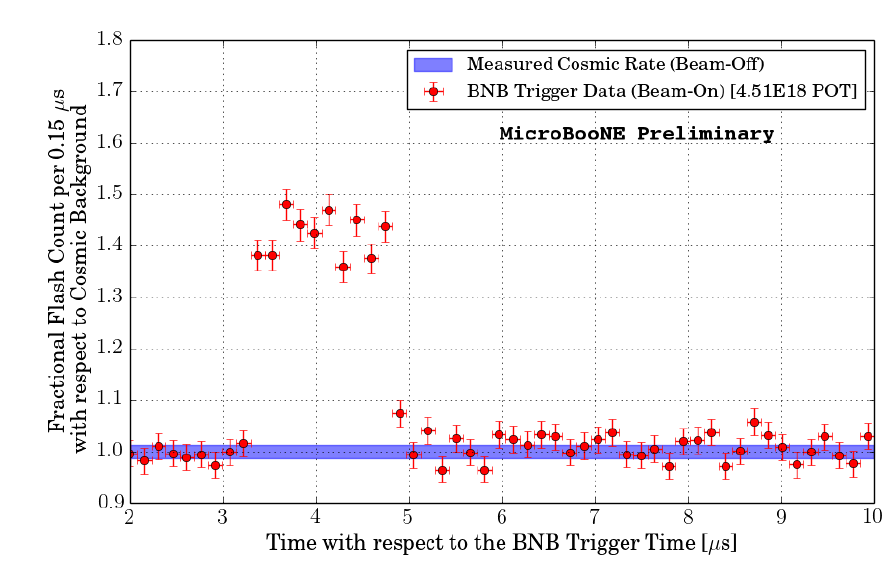
\includegraphics[width=.6\textwidth]{figs/opticaltrigger.png}
\caption{Time distribution of reconstructed optical flashes with a PE value of 50 or more for a sample of BNB unbiased triggered events.}
\label{fig:optrig}
\end{figure}

Figure \ref{fig:optrig} shows the time distribution of reconstructed optical flashes using the BNB continuous stream. You can see a clear excess in coincidence with the expected arrival time of neutrinos. The same flash reconstruction that was used in the cc-inclusive filter detailed here was used to create this plot in data.
\subsection{Beam Window}

\begin{figure}[htp!]
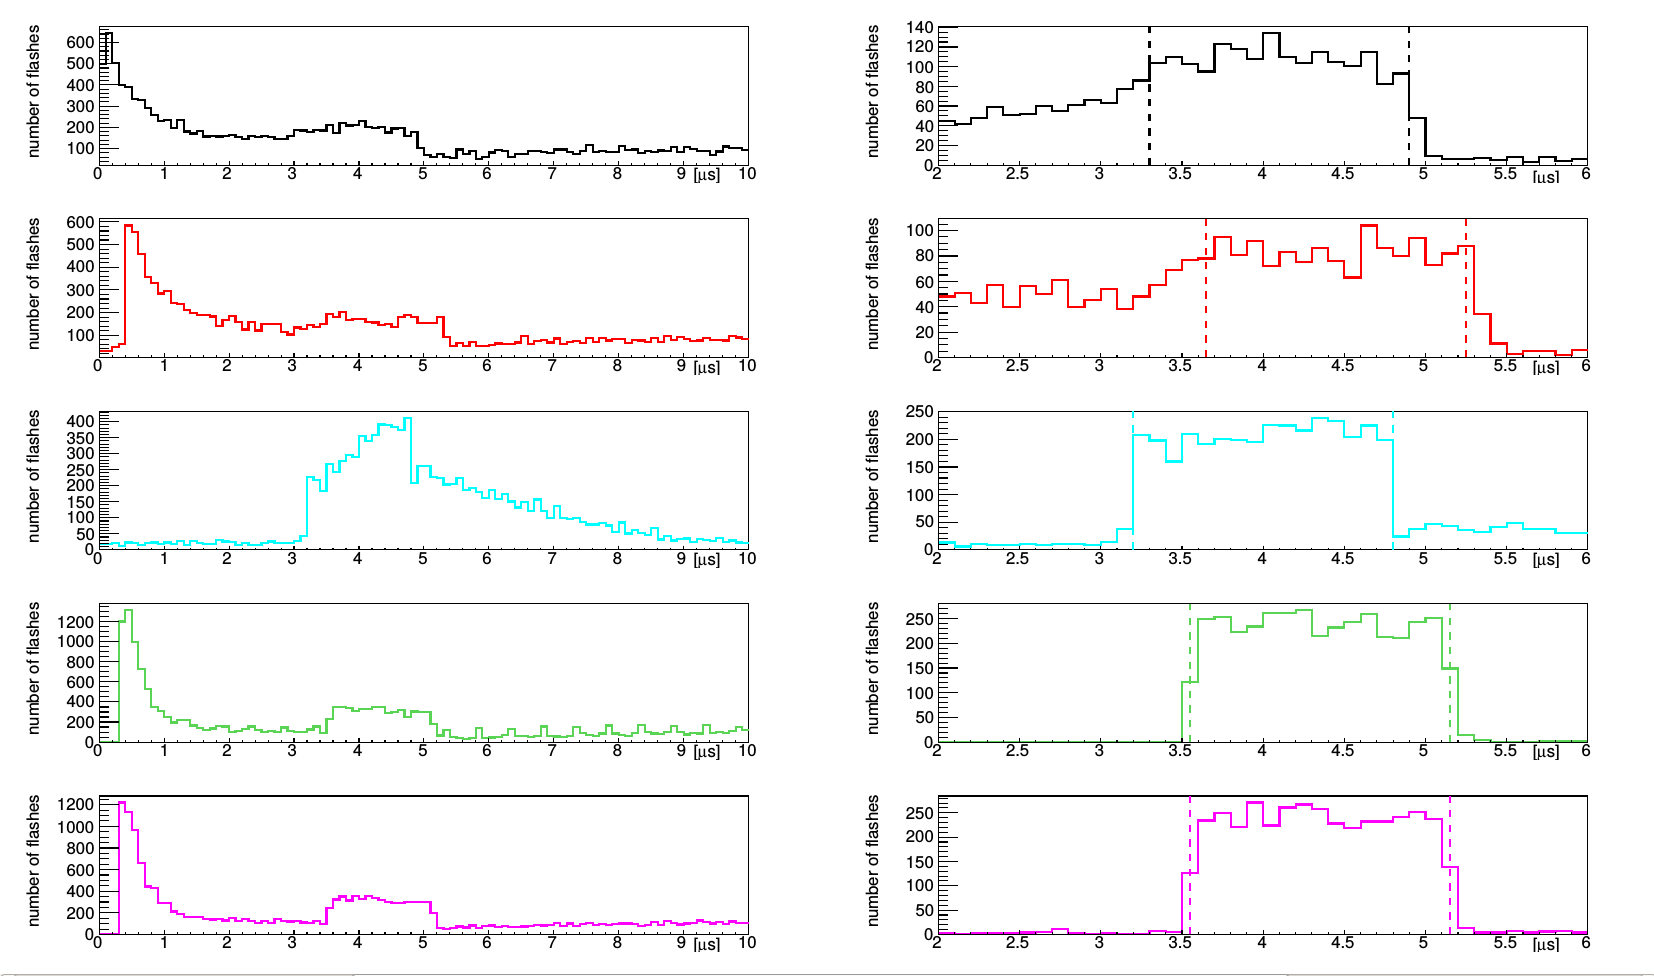
\includegraphics[width=\textwidth]{figs/flashdist.png}
\caption{Flash time distribution for all flashes (left plot) and flashes > 20PE (right plot). The different curves are as follows: on-beam data (black), off-beam data (red), CORSIKA inTime MC (light blue), BNB only MC (green), and BNB+Cosmic MC (purple). The dashed vertical lines mark the time window that was chosen for each sample}
\label{fig:beamwindow}
\end{figure}

Figure \ref{fig:beamwindow} shows the distribution of flashes for on-beam, off-beam and various MC samples. The software trigger has been applied to these samples. The pile-up seen just after 0 $\micro s$ is a feature of the flash finding algorithm and consists of low PE flashes and is removed in the second column of distributions with a low 20 PE threshold cut. The plots show that the time window for the distributions are shifted a small amount from each-other. This is caused by different hardware configurations per sample. Using these distributions, the windows chosen per sample are as follows:
\begin{itemize}
\item{On-Beam: 3.3 to 4.9 $\micro s$}
\item{Off-Beam: 3.65 to 5.25 $\micro s$} 
\item{CORSIKA inTime: 3.2 to 4.8 $\micro s$}
\item{BNB only: 3.55 to 5.15 $\micro s$} 
\item{BNB+Cosmic: 3.55 to 5.15 $\micro s$} 
\end{itemize}
Each window has a width of 1.6 $\micro s$. 


\section{TPC Reconstruction}
\begin{figure}[htp!]
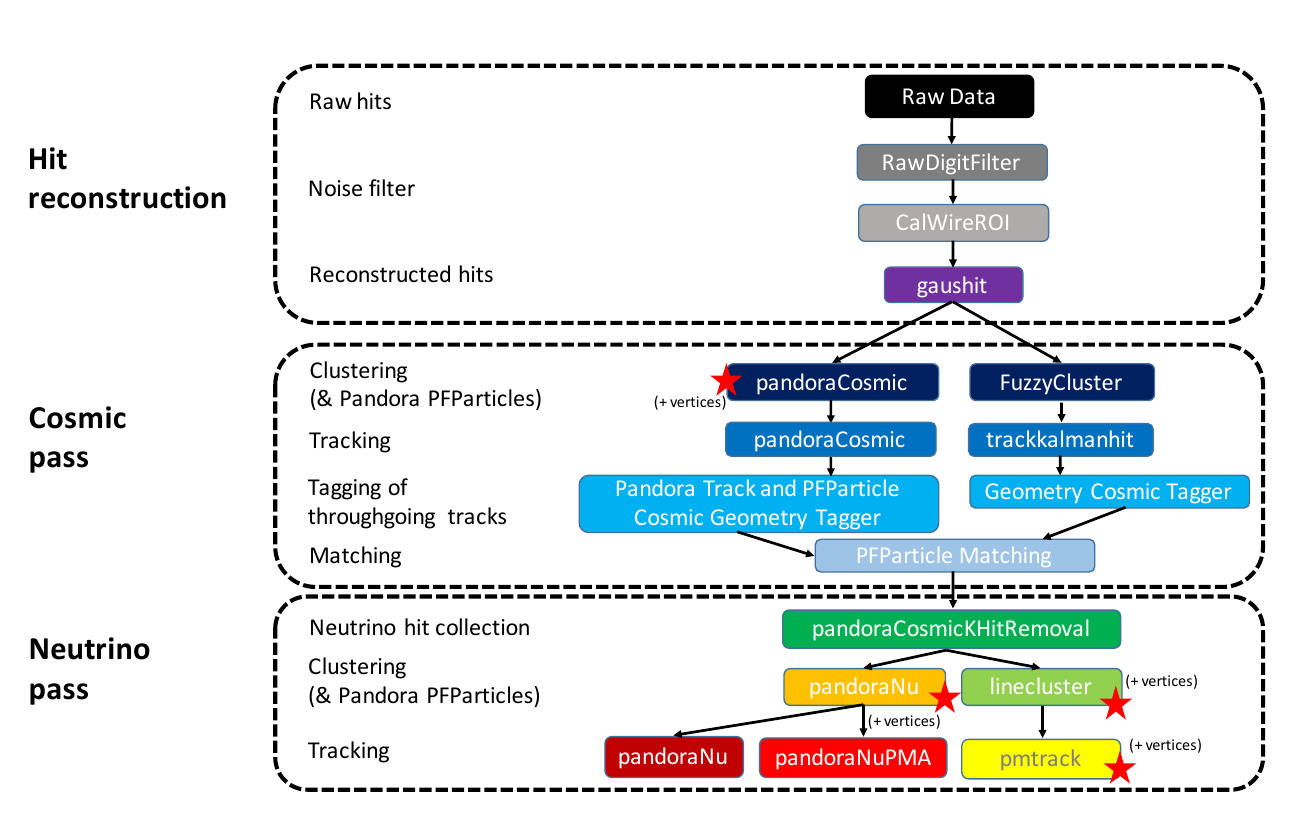
\includegraphics[width=\textwidth]{figs/reconstructionchain.png}
\caption{Reconstruction chain run on both data and MC. The red stars mean that the algorithm returns reconstructed 3D vertices.}
\label{fig:recochain}
\end{figure}

Figure \ref{fig:recochain} summarizes the reconstruction chain applied to both MC and data for this analysis. After the hit reconstruction, a cosmic pass is applied which removes all hits associated to through-going tracks. A description of these TPC reconstruction algorithms will be detailed below.
\subsection{Hit Reconstruction}
The waveforms used for hit reconstruction consist of charge deposited on the sense wire in drift time. The first step in hit reconstruction is to pass the waveforms through a filtering algorithm to filter out the noise introduced from the electronics. The input waveforms are also truncated from 9600 time ticks to 6400 time ticks in this first step to reduce the data footprint of these waveforms. 

Once noise filtering is complete, a deconvolution algorithm is applied to the waveforms to remove the drift field and electronics response, therefore leaving only the ionized electrons kicked off the argon atoms by an incident track. During this process, Region of Interests (ROI) are identified and cut out of the waveforms to further reduce the data volume. 

The hit finding algorithm then finds candidate peaks in these ROI's and fits the peaks to Gaussian curves. These Gaussian shaped peaks are now called hits and represent the charge deposition on a wire by the incoming track. These hit objects have a peak time and width and are the basic object input to further algorithms down the reconstruction chain.   
\subsection{Clustering}
There are multiple clustering algorithms used in this analysis. The main purpose of all the clustering algorithms is to associate hits together in 2D space to create objects like tracks, vertices and showers. For the fuzzy cluster algorithm, three steps are used to achieve this. The first step is to associate hits to each-other using a fuzzy clustering algorithm which gives each hit a degree of belonging to the cluster. Second, a Hough transform is used to find hits associated to candidate tracks and showers within each of the clusters found in the first step. The last step merges smaller candidate tracks and showers into large clusters. The last step also associates unclustered hits into nearby objects which helps shower reconstruction. The result is a set of clusters made up of associate hits that represent tracks or showers per plane. 

The pandora algorithm utilizes it's own clustering algorithm and will be detailed in the next section. The last clustering algorithm is called linecluster. The linecluster algorithm reconstructs 2D linear clusters per plane by fitting a line onto nearby hits which is then extrapolated to neighboring wires. 2D vertices are found per plane by using the intersection points of the ends of nearby clusters. These 2D vertices are then matched in time across all three planes to get a 3D vertex in space.  
\subsection{Pandora}

\subsection{Trackkalmanhit}
The trackkalmanhit algorithm takes 2D clusters returned from the fuzzy cluster algorithm and outputs track objects. There are no hierarchy structure as it is in pandora, each track is independent. There also is no vertex reconstruction with this algorithm as well.
\subsection{Cosmic Hit Removal}
The Pandora algorithm is applied to the events twice, the first to remove downward going tracks primarily from cosmic ray muon like particles. The second pass only runs on a subset of hits that aren't associated with cosmic ray muon tracks. 

After the first pass, the output of PFParticle hierarchy is then passed to a cosmic ray tagger to look through all hits to determine start and end points. If the start or end point trajectories are consistent with entering or exiting the TPC, then these hits are removed from the second pass. Hits are considered entering or exiting the TPC if the drift time are outside of the neutrino drift window or outside of the fiducial volume of the TPC. The fiducial volume was based on a montecarlo study and is 20 cm from the top or bottom of the TPC and 10 cm from the TPC ends. Hits associated with candidate cosmic  ray tracks are removed from the input hit collection and the remaining hits are passed to the neutrino optimized pass of Pandora.


\subsection{Projection Matching Algorithm}
The projection matching algorithm (PMA) was inherited from ICARUS and has been implemented in LArSoft. PMA differs from traditional LArSoft 3D reconstruction algorithms. Most 3D reconstruction attempts to match 2D objects from all three planes by drift time, while the PMA algorithm projects a track hypothesis on each plane then the distance between this projection and the hits on each plane is minimized simultaneously. More information can be found in \cite{PMA}.
\section{Event Selection}
The first requirement for selecting $\nu_{\mu}$ CC events is that the event has at least one scintillation light flash in the beam trigger window with more than 50 PE on all PMTs combined. From the flashes that pass, the most intense is chosen and considered to be originating from a neutrino interaction and will be the only flash used in further cuts. 

Vertices are then required to have at least one reconstructed track start or endpoint within a 5 cm radius. Showers associated with a vertex do not pass this cut. All tracks associated with a vertex are then used to calculate a track length weighted average of the $\theta$-angle. Of all the vertices that do pass, only the vertex with the most forward going $\theta$-angle average of all associated tracks is considered the neutrino vertex candidate. The most forward going $\theta$-angle average is chosen by picking the largest track range weighted average of $|cos(\theta)|$, seeing as $cos(\theta)=1$ is the beam direction. Next, it is required that the reconstructed neutrino vertex candidate be within the fiducial volume as well as within the drift time starting at $t_0$. The fiducial volume boundaries chosen are 10 cm from the edges of the TPC in x and z which is the drift direction and beam direction respectively, and 20 cm from the edges of the TPC in y which is the vertical direction. For all further cuts, only the longest track associated with the neutrino vertex candidate and this track is assumed to be the muon candidate of the neutrino event.

The next cut requires the position of the flash in the z-direction and the track z-projection to be compared. This basic flash matching algorithm is rudimentary and a placeholder for a more sophisticated algorithm. The z-position of the flash needs to be within 80 cm to the z-positions of track start or endpoints. If the flash is between the track start and endpoint, the distance of the flash to the track is considered to be 0 cm. 

Lastly, the track needs to be fully contained within the fiducial volume and have a track range greater than 75 cm. The range is the 3D distance between the track's start and endpoint. The length cut was optimized to remove NC background that contain a pion due to the pion interaction rate to be \sim 70 cm. A track that makes all the cuts is considered to be the muon of a $\nu_{\mu}$ CC event. The list of cuts for this selection is described below:
\begin{enumerate}
\item At least one falsh > 50 PE within the beam gate.
\item At least one track witin 5 cm around a vertex.
\item Vertex with flattest tracks is chosen to be vertex candidate.
\item Vertex candidate in fiducial volume.
\item Longest track associated with vertex candidate is chosen to be track candidate.
\item Longest track is within 80 cm (z-axis only) of the flash.
\item Longest track is fully contained.
\item Longest track is greater than 75 cm.
\end{enumerate}

The event selection scheme can also be seen in figure \ref{fig:selection}. Table \ref{table:mc} lists the passing rates for MC events for the selection scheme describes above. Table \ref{table:data} lists the passing rates for on-beam and off-beam data for the selection scheme. The normalization factors applied between on-beam and off-beam data are described in section \ref{section:normalize}.
\begin{figure}[htp!]
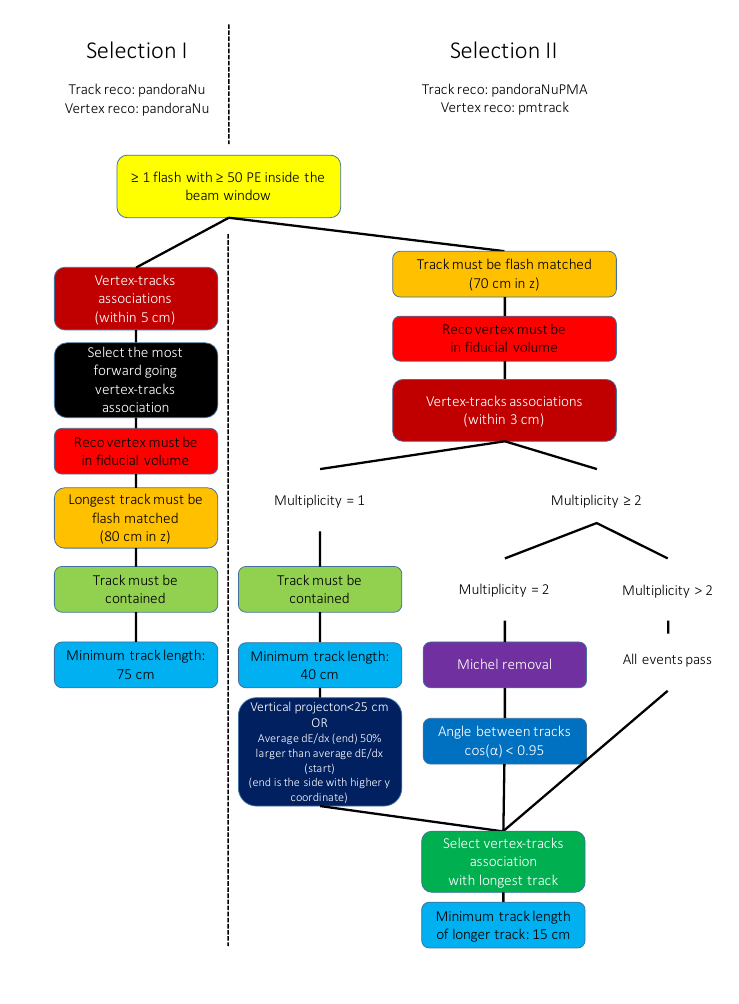
\includegraphics[width=\textwidth]{figs/selection.png}
\caption{Event selection diagram for selection I and selection II. This analysis focused on optimizing selection I. Boxes with the same color across the two selections symbolize similar cuts.}
\label{fig:selection}
\end{figure}

\begin{table}
\begin{center}
\begin{tabular}{c |c |c | c}
\hline
& \vline  BNB+Cosmic  & \vline Cosmic Only  & \vline Signal:Cosmic Only \vline \\
& \vline  Selection	MC-Truth  & \vline & \\
Generated Events 			& $191362	     	45273 		 $	& $4804 	   $	& $1:22$ \\
\geq 1 flash with \geq 50 PE 		& $136219 (71\%/71\%)	44002 (97\%/97\%)$ 	& $2970 (62\%/62\%)$ 	& $1:14$ \\
\geq 1 track within 5 cm of vertex 	& $135830 (99\%/71\%)	43974 (99\%/97\%)$ 	& $2975 (99\%/62\%)$ 	& $1:14$ \\
vertex candidate in FV
flash matching of longest track
track containment
track \geq 75 cm
\end{tabular}
\caption{Passing rates for 2D cluster cuts for neutrino on MC set and a cosmic only MC set. First column shows event rates with no cuts applied to both sets. Columns two and three show event rates after primary and secondary cuts are applied. Line three shows the seccond line scaled with the flash finding factor of 0.008. All events are normalized to per day assuming we are running at 5 Hz.}
\label{table:mc}
\end{center}
\end{table}
The resulting neutrino/cosmic event rate per day is shown in table \ref{table:eventrate}. Figures \ref{fig:2dprimarycut} and \ref{fig:2dsecondarycuts} shows the percentages of clusters that pass each primary and secondary cuts.     
%\section{The importance of $\mu/\pi$ separation}
